%!TEX root = ../main.tex
%%%%%%%%%%%%%%%%%%%%%%%%%%%%%%%%%%
% Links:
%
% Difficulty: Companies: 
%%%%%%%%%%%%%%%%%%%%%%%%%%%%%%%%%%


%\begin{figure} \centering
%   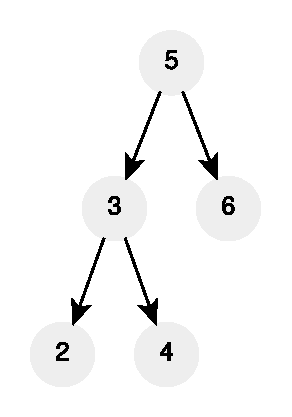
\includegraphics[width=\textwidth]{sources/remove_duplicated_sorted_array_inplace/images/example1}
%   \caption[Sample short cpation]{Sample Caption}.
%   \label{fig:remove_duplicated_sorted_array_inplace:example1} \end{figure}

\chapter{Remove duplicates in sorted array}
\label{ch:remove_duplicated_sorted_array_inplace}
\section*{Introduction}
Sorting and duplicates are the bread and butter of coding interview questions. There are countless
problems that asks you to perform various operations where you either have some sort of sorted input
and involving duplicates. In the problem described in this chapter we are going to investigate how
we can remove duplicates from an already sorted collection of elements. This problem is trivially
solvable when you can use linear space, but solving it such that the operations are done in-place
and by only using constant time is going to be slightly more challenging.


\section{Problem statement}
\begin{exercise}
Write a function that take a sorted array $I$ as input and  returns the number of unique elements
$u$ in it. The function should also cause all the unique elements of $I$ to appear in the first $u$
positions.

\label{example:remove_duplicated_sorted_array_inplace:exercice1}

	%example1
	\begin{example}
		\label{example:remove_duplicated_sorted_array_inplace:example1}
		\hfill \\
		Given $I=\{1,1,2,2,3,3,4,5,6,6,6,6,7\}$ the function returns $7$ and $I$ is rearranged such
		that itself first $7$ elements are $\{1,2,3,4,5,6,7\}$.				
	\end{example}

	%example2
	\begin{example}
		\label{example:remove_duplicated_sorted_array_inplace:example2}
		\hfill \\
		Given $I=\{1,2,3,4\}$ the function returns $4$ and $I$ is rearranged such that its first $4$
		elements are $\{1,2,3,4\}$.	
	\end{example}
\end{exercise}

\section{Clarification Questions}

\begin{QandA}
	\item Is it guaranteed for the input array to  contain integers? 
	\begin{answered}
		\textit{Yes you can assume $I$ is an array of integers. But if you are free to produce a generic solution.}
	\end{answered}	
\end{QandA}

\section{Discussion}
\label{remove_duplicated_sorted_array_inplace:sec:discussion}
This problem is remarkably similar to what how the function \inline{std::unique} from the STL
library behaves. Such function does not really remove any elements from the input collection, but
what it does instead is rearranging the elements such that the initial collection is divided into
two parts:
\begin{enumerate}
	\item the first containing only the unique elements
	\item the second where the duplicate elements are moved to (possibly empty)
\end{enumerate}
This function is often used in pair with \inline{std::erase} to delete the second part of the newly
arranged collection. Listing \ref{list:remove_duplicated_sorted_array_inplace_stl} shows how you can
solve this problem with a one-liner solution. Being able to show you can use the standard library to
solve relatively complex problem is a good thing that every interviewer appreciate. However, despite
making a good impression, this is not enough to clear the round just yet as if you use this solution
during an actual interview the interviewer would very likely asks you implement \inline{std::unique}
yourself.

\begin{minipage}{\linewidth}
	\lstinputlisting[language=c++, caption={One-liner solution using \inline{std::unique}.},label=list:remove_duplicated_sorted_array_inplace_stl]{sources/remove_duplicated_sorted_array_inplace/remove_duplicated_sorted_array_inplace_solution3.cpp}
\end{minipage}

As already mentioned in the introduction it is quite easy to implement this problem when you can use
linear additional space. You can think of building a list $U$ of unique elements of $I$ by:
\begin{itemize}
	\item inserting the first element of $I$
	\item insert all the elements at position $k$ s.t. $I_k \neq I_{k+1}$
\end{itemize}
At the end of this process $U$ contains an ordered list of all the unique elements in $I$. All we
have to do is to copy $U$ into the first $|U|$ positions of $|I|$ and return $|U|$. The complexity
of this approach is linear in time and space as in the worst-case read and write all the elements of
$I$ twice. An implementation of this approach is shown in Listing
\ref{list:remove_duplicated_sorted_array_inplace_linearspace}.

\begin{minipage}{\linewidth}
	\lstinputlisting[language=c++, caption={Linear time and space solution using \inline{std::std::unordered_set} to remember what elements have been already encountered.},label=list:remove_duplicated_sorted_array_inplace_linearspace]{sources/remove_duplicated_sorted_array_inplace/remove_duplicated_sorted_array_inplace_solution2.cpp}
\end{minipage}

Despite we cannot do much better than spending linear time, we can improve on the space and bring it
down to constant. The key idea is that because the array is sorted, equal elements will be one next
to the other, forming clusters of the same value. Eventually $I$ has to be logically divided into
two subarrays where we only care about the content of the first-part only containing the unique
elements. We have no constraints on the second half. The algorithm proposed in this Section will
build the first half of $I$ one element at a time.  This can be achieved by looping through the
elements of $I$ and keeping track of two pointers:
\begin{itemize}
	\item $x$: a pointer to the last element of the first part of $I$
	\item $y$ a pointer to the next element to be processed 
\end{itemize}
When the element pointed by $y$ is different to the element pointer by $x$ we know that we can add
$y$ to the first part of $I$. We can do that by copying $I_y$ into $I_{x+1}$ and incrementing both
$y$ and $x$ so that the next comparison would be among the last inserted element and the next
element to be processed. If they are equal, the first part of $I$ is not going to grow and we can
safely ignore the element pointed by $y$ as we already have an instance of it in the first half of
$I$.

When all the element of $I$ are processed ($y \geq |I|$) the algorithm can be stopped. At this point
we know that $x$ is marking the end of the part of $I$ containing only unique elements. All we have
to do is calculate its length and return it. Listing
\ref{list:remove_duplicated_sorted_array_inplace} shows an implementation of such idea. As already
stated before, its complexity is linear in time and constant in space.
Notice that because we do not have to maintain the state of the elements of $I$ after the point where all the unique elements are
we can use \inline{std::move} to potentially avoid expensive copies.

\begin{minipage}{\linewidth}
	\lstinputlisting[language=c++, caption={Linear time constant space solution.},label=list:remove_duplicated_sorted_array_inplace]{sources/remove_duplicated_sorted_array_inplace/remove_duplicated_sorted_array_inplace_solution1.cpp}
\end{minipage}



\begin{figure}
	\centering
	\vspace*{0.0in}
	\begin{subfigure}[t]{0.49\textwidth}
		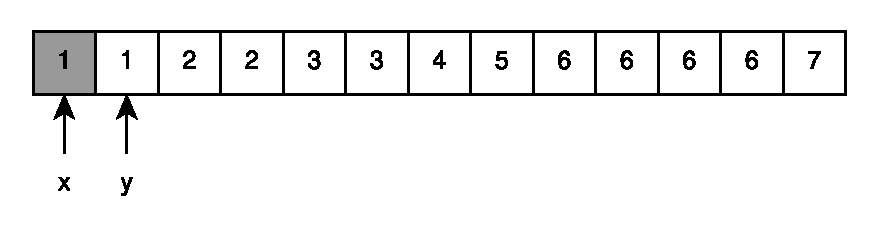
\includegraphics[width=1\linewidth]{sources/remove_duplicated_sorted_array_inplace/images/example1_1}
		\vspace*{-8mm}
		\caption{$I_x = I_y$. $y$ moved forward.}
		\label{fig:remove_duplicated_sorted_array_inplace:example1_1}
	 \end{subfigure}
	 \hfill
	 \begin{subfigure}[t]{0.49\textwidth}
		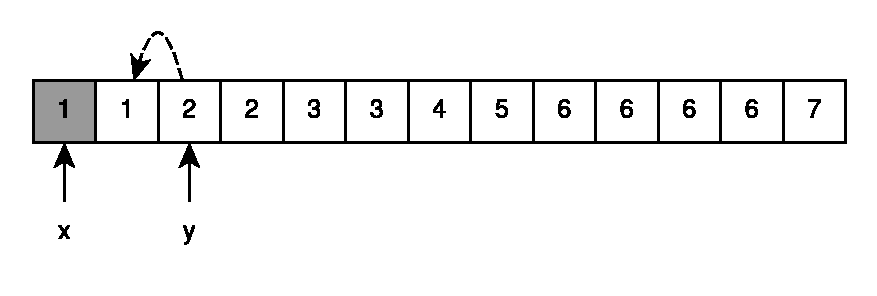
\includegraphics[width=1\linewidth]{sources/remove_duplicated_sorted_array_inplace/images/example1_2}
		\vspace*{-8mm}
		\caption{$1 = I_x \neq I_y = 2$. $I_y$ copied into $I_{x+1}$. $y$ and $x$ are moved forward.}
		\label{fig:remove_duplicated_sorted_array_inplace:example1_2}
	 \end{subfigure}
	 \hfill
	 \begin{subfigure}[t]{0.49\textwidth}
		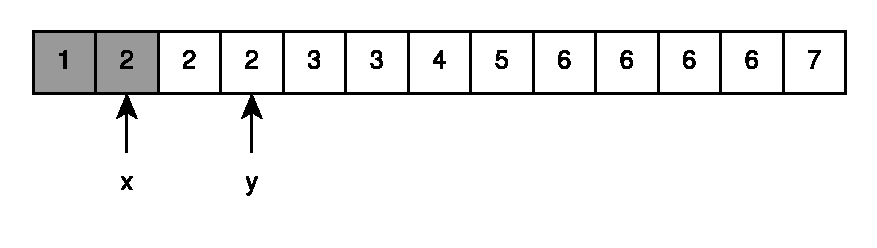
\includegraphics[width=1\linewidth]{sources/remove_duplicated_sorted_array_inplace/images/example1_3}
		\vspace*{-8mm}
		\caption{$I_x = I_y$. $y$ only moved forward.}
		\label{fig:remove_duplicated_sorted_array_inplace:example1_3}
	 \end{subfigure}
	 \hfill
	 \begin{subfigure}[t]{0.49\textwidth}
		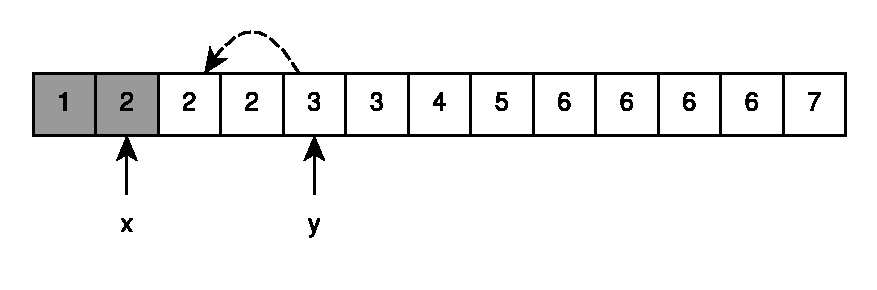
\includegraphics[width=1\linewidth]{sources/remove_duplicated_sorted_array_inplace/images/example1_4}
		\vspace*{-8mm}
		\caption{$2 = I_x \neq I_y = 3$. $I_y$ copied into $I_{x+1}$. $y$ and $x$ are moved forward.}
		\label{fig:remove_duplicated_sorted_array_inplace:example1_4}
	 \end{subfigure}
	 \hfill
	 \begin{subfigure}[t]{0.49\textwidth}
		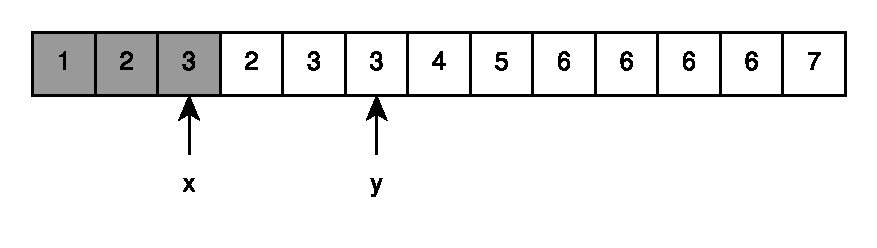
\includegraphics[width=1\linewidth]{sources/remove_duplicated_sorted_array_inplace/images/example1_5}
		\vspace*{-8mm}
		\caption{$I_x = I_y$. $y$ moved forward.}
		\label{fig:remove_duplicated_sorted_array_inplace:example1_5}
	 \end{subfigure}
	 \hfill
	 \begin{subfigure}[t]{0.49\textwidth}
		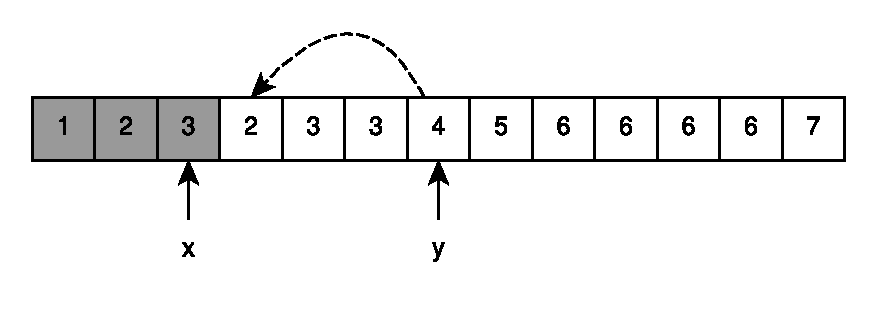
\includegraphics[width=1\linewidth]{sources/remove_duplicated_sorted_array_inplace/images/example1_7}
		\vspace*{-8mm}
		\caption{$3 = I_x \neq I_y = 4$. $I_y$ copied into $I_{x+1}$. $y$ and $x$ are moved forward.}
		\label{fig:remove_duplicated_sorted_array_inplace:example1_6}
	 \end{subfigure}
	 \hfill
	 \begin{subfigure}[t]{0.49\textwidth}
		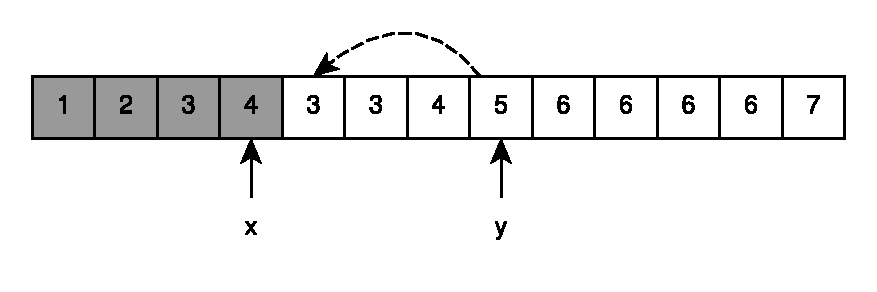
\includegraphics[width=1\linewidth]{sources/remove_duplicated_sorted_array_inplace/images/example1_8}
		\vspace*{-8mm}
		\caption{$4 = I_x \neq I_y = 5$. $I_y$ copied into $I_{x+1}$. $y$ and $x$ are moved forward.}
		\label{fig:remove_duplicated_sorted_array_inplace:example1_6}
	 \end{subfigure}
	 \hfill
	 \begin{subfigure}[t]{0.49\textwidth}
		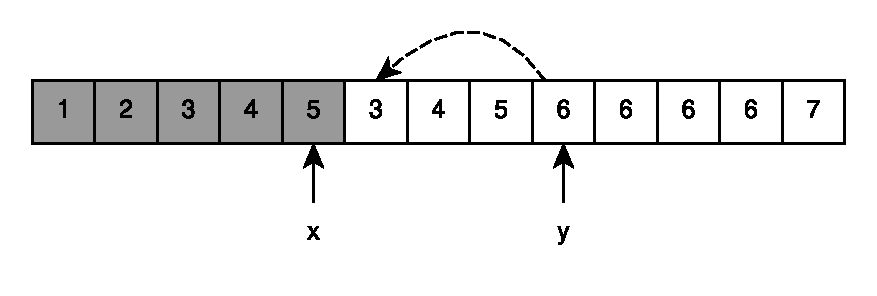
\includegraphics[width=1\linewidth]{sources/remove_duplicated_sorted_array_inplace/images/example1_10}
		\vspace*{-8mm}
		\caption{$5 = I_x \neq I_y = 6$. $I_y$ copied into $I_{x+1}$. $y$ and $x$ are moved forward.}
		\label{fig:remove_duplicated_sorted_array_inplace:example1_6}
	 \end{subfigure}
	 \hfill
	 \begin{subfigure}[t]{0.49\textwidth}
		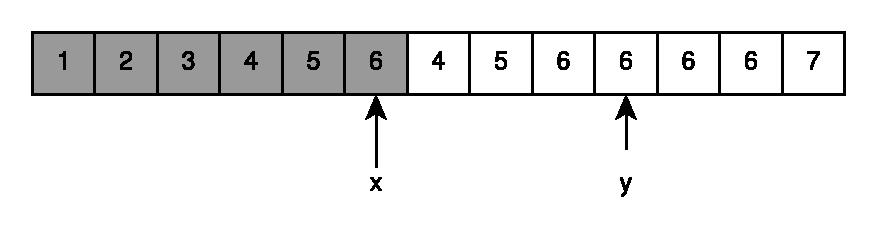
\includegraphics[width=1\linewidth]{sources/remove_duplicated_sorted_array_inplace/images/example1_11}
		\vspace*{-8mm}
		\caption{$I_x = I_y$. $y$ moved forward.}
		\label{fig:remove_duplicated_sorted_array_inplace:example1_6}
	 \end{subfigure}
	 \hfill
	 \begin{subfigure}[t]{0.49\textwidth}
		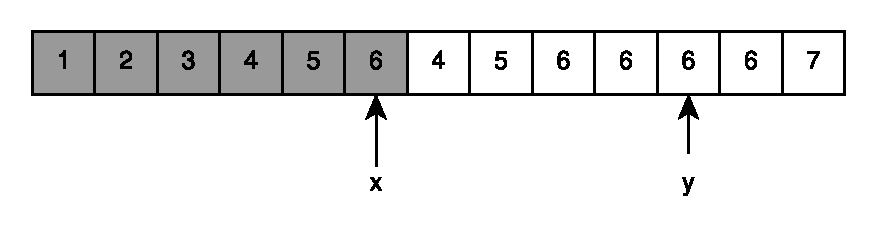
\includegraphics[width=1\linewidth]{sources/remove_duplicated_sorted_array_inplace/images/example1_12}
		\caption{$I_x = I_y$. $y$ moved forward.}
		\label{fig:remove_duplicated_sorted_array_inplace:example1_6}
	 \end{subfigure}
	 \hfill
	 \begin{subfigure}[t]{0.49\textwidth}
		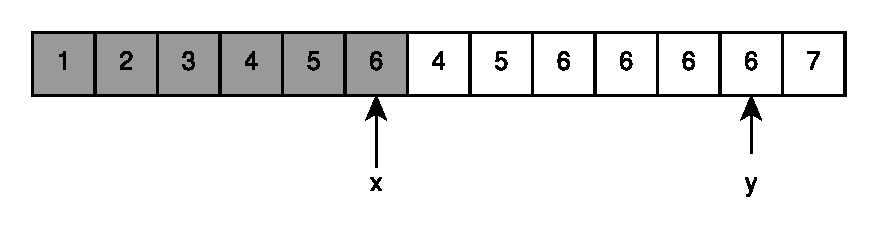
\includegraphics[width=1\linewidth]{sources/remove_duplicated_sorted_array_inplace/images/example1_13}
		\vspace*{-8mm}
		\caption{$I_x = I_y$. $y$ moved forward.}
		\label{fig:remove_duplicated_sorted_array_inplace:example1_6}
	 \end{subfigure}
	 \hfill
	 \begin{subfigure}[t]{0.49\textwidth}
		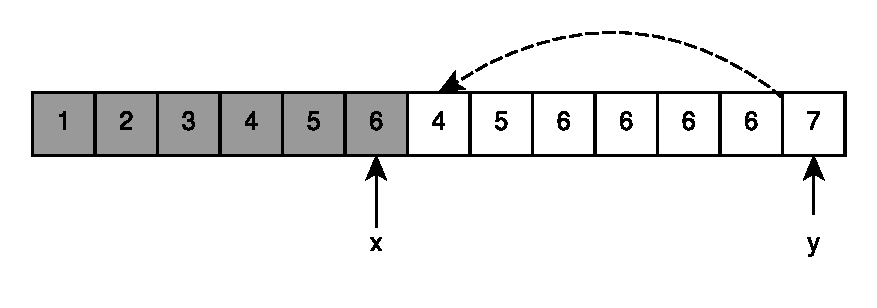
\includegraphics[width=1\linewidth]{sources/remove_duplicated_sorted_array_inplace/images/example1_14}
		\vspace*{-8mm}
		\caption{$6 = I_x \neq I_y = 7$. $I_y$ copied into $I_{x+1}$. $y$ and $x$ are moved forward.}
		\label{fig:remove_duplicated_sorted_array_inplace:example1_6}
	 \end{subfigure}
	 \hfill
	 \begin{subfigure}[t]{0.49\textwidth}
		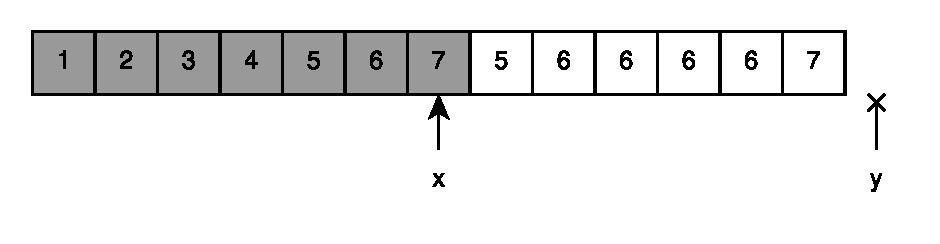
\includegraphics[width=1\linewidth]{sources/remove_duplicated_sorted_array_inplace/images/example1_15}
		\vspace*{-8mm}
		\caption{$y$ is outside the range of valid elements of $I$. The algorithm stops.}
		\label{fig:remove_duplicated_sorted_array_inplace:example1_6}
	 \end{subfigure}
\caption{Execution of the algorithm implementd in Listing
 \ref{list:remove_duplicated_sorted_array_inplace} on the input of the Example
 \ref{example:remove_duplicated_sorted_array_inplace:example1}. The shaded part of the array
 contains all the unique elements processed so far. $x$ is a pointer to the last element of this
 sequence. $y$ is a pointer to the element currently processed.}
\label{fig:remove_duplicated_sorted_array_inplace:example1_process}
\end{figure}

\section{Common Variations}
\subsection{Max $2$ duplicates allowed}
This is a common variation of the main problem described earlier in this Chapter where the task 
we have to accomplish is almost identical except this time each element can appears at most 
twice in the final rearrangements of $I$.
\begin{exercise}
	Write a function that given a sorted array $I$ removes all the 
	duplicates in such a way an element appears at most twice and at with all the valid elements being located at the beginning of the $I$ itself.
	The function returns the number of valid elements left in $I$.
	
	\label{example:remove_duplicated_sorted_array_inplace:exercice2}
	
		%example1
		\begin{example}
			\label{example:remove_duplicated_sorted_array_inplace_variation1:example1}
			\hfill \\
			Given $I=\{1,1,2,2,3,3,4,5,6,6,6,6,7\}$ the function returns $11$ and $I$ is rearranged such
			that itself first $11$ elements are $\{1,1,2,2,3,3,4,5,6,6,7\}$.				
		\end{example}
	
		%example2
		\begin{example}
			\label{example:remove_duplicated_sorted_array_inplace_variation1:example2}
			\hfill \\
			Given $I=\{1,2,3,4\}$ the function returns $4$ and $I$ is rearranged such that its first $4$
			elements are $\{1,2,3,4\}$.	
		\end{example}
	\end{exercise}

\subsection{Discussion}

\lstinputlisting[language=c++, caption={Linear time constant space solution.},label=list:remove_duplicated_sorted_array_inplace]{sources/remove_duplicated_sorted_array_inplace/remove_duplicated_sorted_array_inplace_solution4.cpp}

\subsection{Max $k$ duplicates allowed}
This variation is also a quite common, and it is basically a generalization of problems above where this time each element can appear $k$ times.
When $k= 1$ and $k=2$ this problem is equivalent to the Problems \ref{example:remove_duplicated_sorted_array_inplace:exercice1} and \ref{example:remove_duplicated_sorted_array_inplace:exercice2}, respectively.
The solution for this variation is not discussed here as it can be trivially derived from the solution to the Problem \ref{example:remove_duplicated_sorted_array_inplace:exercice1}.
\begin{exercise}
	Write a function that given a sorted array $I$ removes all the 
	duplicates in such a way an element appears at most $k$ times with all the valid elements being located at the beginning of the $I$ itself.
	The function returns the number of valid elements left in $I$.
	
	\label{example:remove_duplicated_sorted_array_inplace_variation:exercice3}
	
		%example1
		\begin{example}
			\label{example:remove_duplicated_sorted_array_inplace_variation2:example1}
			\hfill \\
			Given $I=\{1,1,2,2,3,3,4,5,6,6,6,6,7\}$ and $k=3$ the function returns $12$ and $I$ is rearranged such
			that itself first $1$ elements are $\{1,1,2,2,3,3,4,5,6,6,6,7\}$. Notice the extra $6$ w.r.t. the Example \ref{example:remove_duplicated_sorted_array_inplace_variation1:example1}.
		\end{example}
	
		%example2
		\begin{example}
			\label{example:remove_duplicated_sorted_array_inplace_variation2:example2}
			\hfill \\
			Given $I=\{1,1,1,1,1,1,1,2,2,3,3,3,4,4\}$ and $k=5$ the function returns $13$ and $I$ is rearranged such that its first $13$
			elements are $\{1,1,1,1,1,2,2,3,3,3,3,4,4\}$.	
		\end{example}
	\end{exercise}